\vspace{-10ex}%
\rule{\textwidth}{0.3pt}
\vspace{5ex}

\textit{
This chapter will introduce the reader to the problem formulation and the underlaying principles taken into account. The priciple of radio communication and the important steps involved in developing a new product prototype will be presented. Basic information of the communication and programming will also be presented. 
}
\vspace{5ex}



\section{Prototyping}
Much considerations is taken in orderto construct the final product. In this case the final prototype shoud be as small and inexpensive as possible. Some of the design elements of this prototype is directly related to this. Some basic criteriums for manufacturing is taken from the \gls{pcb} suppliers website. These parameters is some industry standards and also from the manufacturers side the limitations for their equipment. Whitout going up in cost but keeping the cost down with no extra price these are the.



\section{PCB}
To get good characteristics of the circuit the system will be produced on a four-layer \gls{pcb}. This have a lot of advatages over a standard two layer board. The four layer design will have a top layer where all the components will be placed, a bottom layer with extra room for tracing tracks and having another ground pylogon. The two inner layers consist of a power plane and a ground layer. Both for easier connecability and also as a good way of making the circuit more resistant to high frequency noise between the traces on the top and bottom layer.



\section{Radio Frequency}
Radio frequenzy are a set frequencies that is used for trancieving and receiving data wirelessly. Radio frequencies begins with at one end of the spectrum where the frequencies is about 100Hz. It contains all the frequencies up to 300Ghz. At 300Ghz the wavelength is 1mm long. Radio frequencies are divided into different bands, all with different caracteristics and areas of implementation. 

\begin{figure}[H] 
	\centering 
	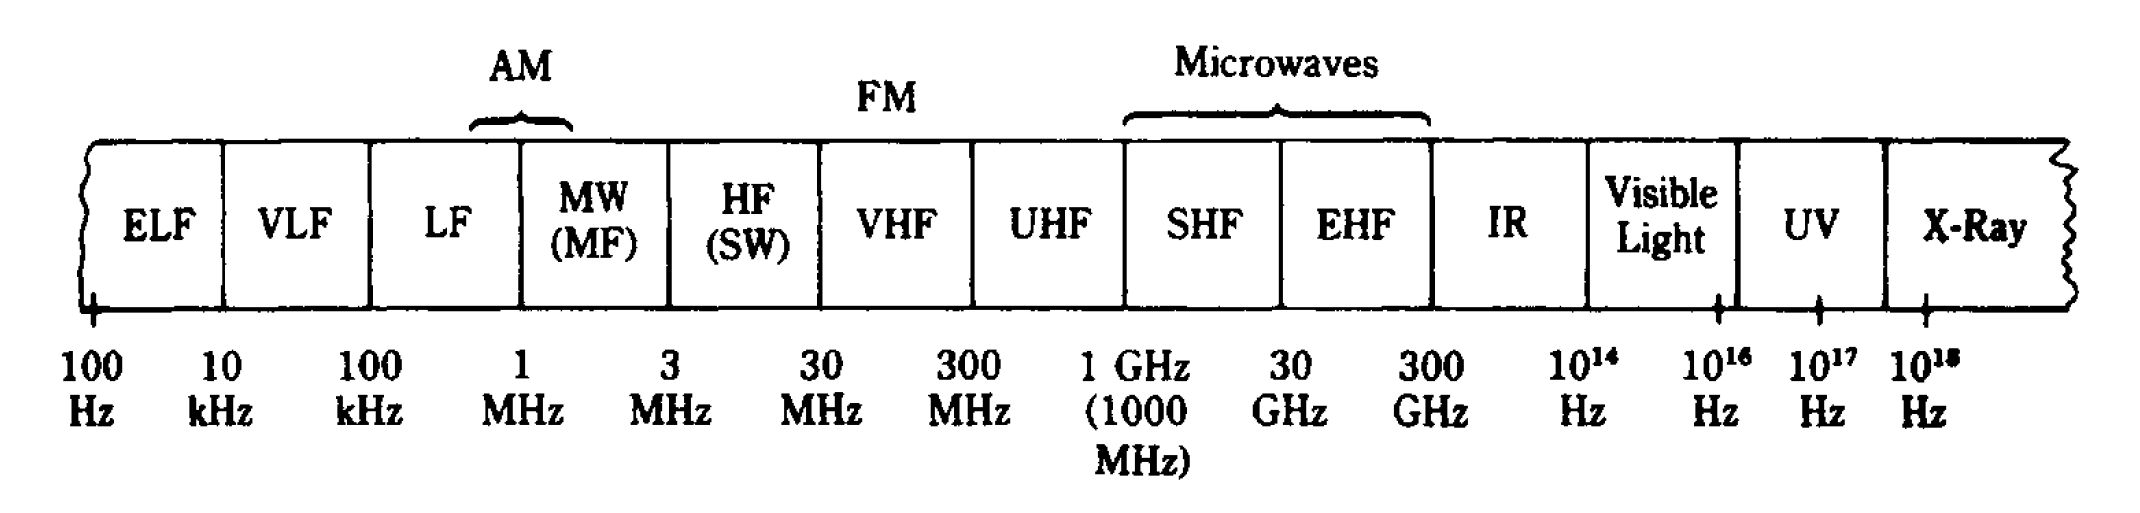
\includegraphics[width=.8\linewidth]{Figures/Full_frequency_band} 
	\captionsource{Electromagnitical frequencies}{RF Circuit Design \cite{rf_circut_design}}
	\label{fig:full_freq_band} 
\end{figure} 

Designing a circuit for radio transmission is a advanced and complex procediur. The high frequencies introduces a lot of intresting phenomenons that need to be considered when construction a circuit in these frequincies. When designing a circuit for RF the components and traces on the \gls{pcb} behaives in a different way and takes on different characteristics than a equal system at lower frequencies. Some of the challenges that arises are described in "Secrets of RF Circuit Design". Stray capacitance is one of the phenomenon that arises when handlig RF. Between conductors, conductors to ground and between components a small capacitance occures when dealing with RF. To ensure a good radio signal  some criterias need to be fulfilled. 
The output signal from the radio tranciever is matched at 50 ohms and this has to be matched with the output stage components. These components commonly is a network of inductors and capacitors .This matching network is described later in this section. 
From different types of radio signal trancievers the type used in this case is determined by the radio \gls{ic}'s manufacturer. %%\cite{silabbsradio}


Another phenomena thats intruduces is the so called skin effect, where the "skin" part comes from the fysical phenomenal thats hapening. When the frequencies rises the resistance in conductors increases with it. The explanation to for this is that current choses the path of least resistance
%High-speed Digital design – Johnson & Graham


Radio frequincies does many things to a board, these problems and apperances most be evaluated and considered.  



"Secrets of RF Circuit Design"
 
\subsection{Chebychev Filter}
The chebychev type of filter is special in the fact that it have a steep fall rate and a high "Q". The Q factor is commonly used in filter design as a function of the length of the stopband through the whole passband.
This makes it very suited for radio designs.. 


\cite{class_e_new}

The class E (CLE) type used here uses switching type of 
The most intresting part of the class E is the fact that up to ideal power eficcianty can be acceived by constructed by this type. Class E makes use f

Stating in the datasheet to the radio \gls{ic} the rough design aspects are defined. From

\section{Radio component}
 The radio module used in this project is from the company Silabs. The chosen radio \gls{ic} have the characteristics that are wanted in this type of product. The radio trasmission used is the earlier explained class E. With this pice the class E is already implemented in the radio as this is widley used today and a very effective radio signal. 
The type of filter used for sending radio signals at \gls{vhf} frequencies is defined in the defined 

\section{MicroControllerUnit}
Every advanced system needs a central processing unit to make all the calculations needed. Why a lot of systems needs some powerful processor this system wich is a bit easier with 
The power consumption is higly dependent on the speed of which the processor is runnig, the faster the more power it consumes and also the slower the less current it will draw. And by the \gls{mcu} beeing the component with the single higest power consumption the speed is set to a speed as low as possible. This low speed is not a concern in this particular system when the operations required is not time or speed sensitive. The voltage supplied to the \gls{mcu} is another parameter that will alter the power consumption. The comonent is a low power model which can handle a lower source voltage. A voltage between 1.7 to 3.6 is required, anything lower will not start the device and anything higer will damage the the part. 
To get the right speed of a crystal we need to get the right product for this particular case. As a crystal 
Many different types of oscillators exists, both internal and external types. 

\section{SPI}
\gls{spi} communication is used to communicate between the \gls{mcu} and other \gls{ic}'s on a circuit board. \cite{pic_spi} The \gls{spi} is 
It uses four wires to communicate and additional one wire for each extra \gls{ic} that is connected. The transmisson works in a synchronous serial maner where each bit is sent one at the time syncronous to a supplied clock signal. Different types of \gls{spi} exists but with the most common beeing the four-wire serial bus. SCL, SDO, SDI and SS is used 

\begin{itemize}[noitemsep]
	\item SCL - Serial CLock, a clock is supplied to synchronise the data transmissions.
	\item SDO - Serial Data Out, Data is sent from this port.
	\item SDI - Serial Data In, Data is transmitted in to this port.
	\item SS - Slave Select, Selects a device for communication.
\end{itemize}
 
Eight bits are sent together to form a package of one byte. Four different modes are available when communicating through \gls{spi}. These modes determine which type of clock signal provided and how the data is sampled in the devices. Two different types of clock signal, one where the clock is pulled high when idle and the other one pulled low when idle. 
The other mode selects the timing of data bits relative to the clock signal. Data is sampled either when the clock signal goes 


\begin{figure}[H]
	\centering
    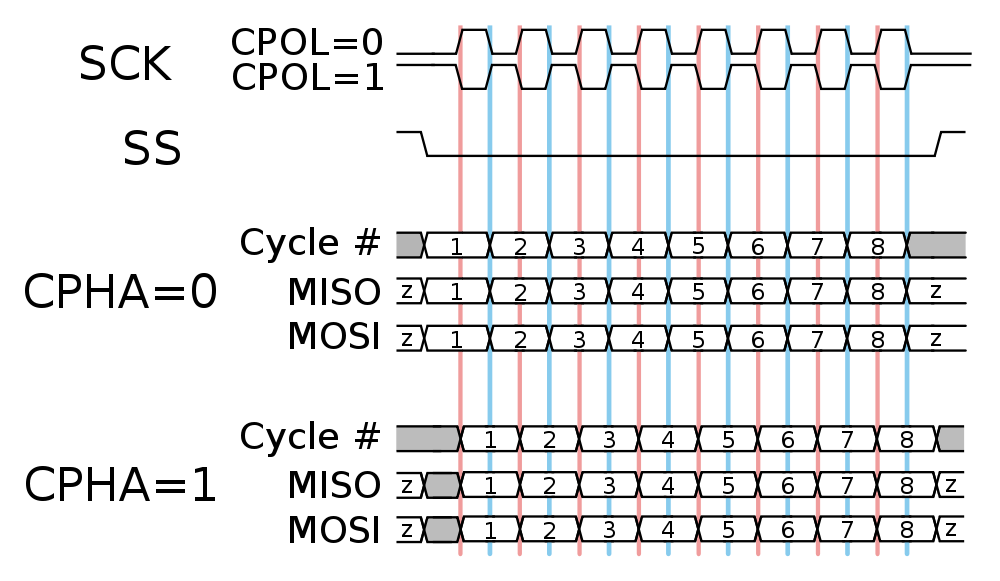
\includegraphics[width=.8\linewidth]{Figures/SPI_timing}
	\captionsource{Timing and modes for a transmission over \gls{spi}}{\url{https://commons.wikimedia.org/wiki/File:SPI_timing_diagram.svg}}
	\label{fig:SPI_timing}
\end{figure}


The interface uses one master device and multiple slaves. The master device handles the communication and supplies the selection of slaves. To enable a connection and choose which slave is used an induvidual slave select must be present. When set, only the choosen slave device is able to communicate.

From the \gls{mcu}'s datasheet the following diagram show in \autoref{fig:PIC_SPI} how the connection works when connection several slave devices.

\begin{figure}[H]
	\centering
    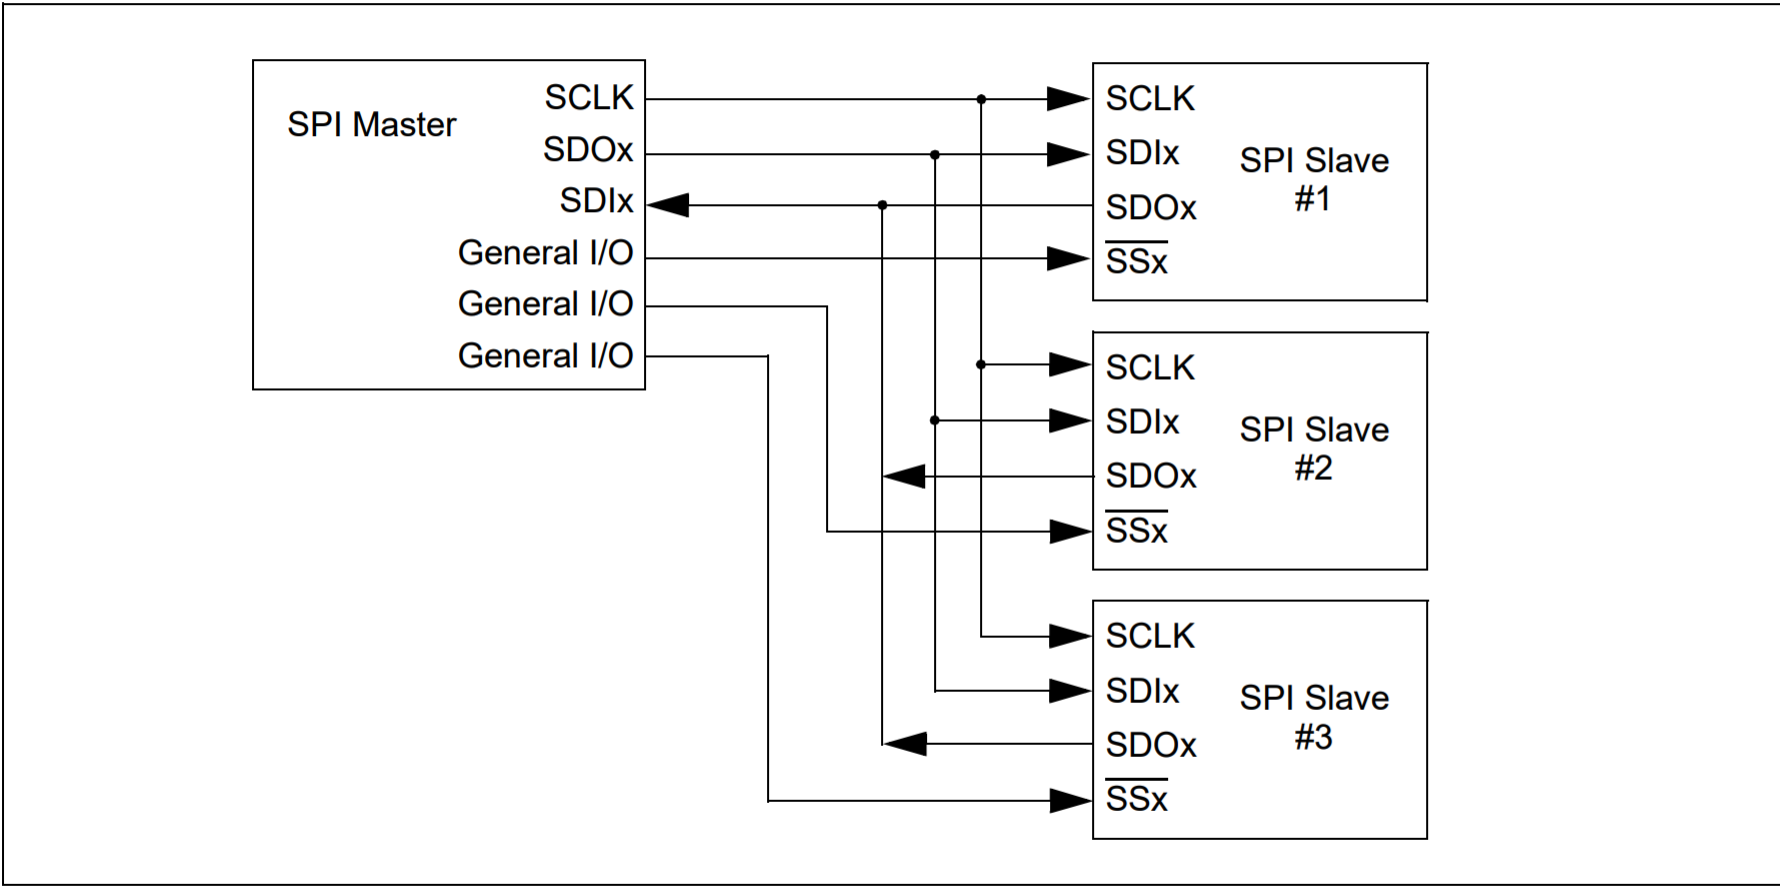
\includegraphics[width=.8\linewidth]{Figures/PIC_SPI}
	\captionsource{SPI master and multiple slave connections}{\url{http://ww1.microchip.com/downloads/en/DeviceDoc/40001412G.pdf}}
	\label{fig:PIC_SPI}
\end{figure}
Data is sent out from the \gls{mcu} at the SDO wire and at the other end connected to the SDI pin of a receiving device. 


\section{I$^2$C}


